\section{Etherless architecture}
Etherless is built upon three components:
\begin{itemize}
	\item \textbf{etherless-cli:} a front-end command line interface that the user uses to interact with the product;
	\item \textbf{etherless-smart:} a smart contract that handles core business logic;
	\item \textbf{etherless-server:} an environment for executing remote functions;
\end{itemize}
\begin{figure}[h]
	\centering
	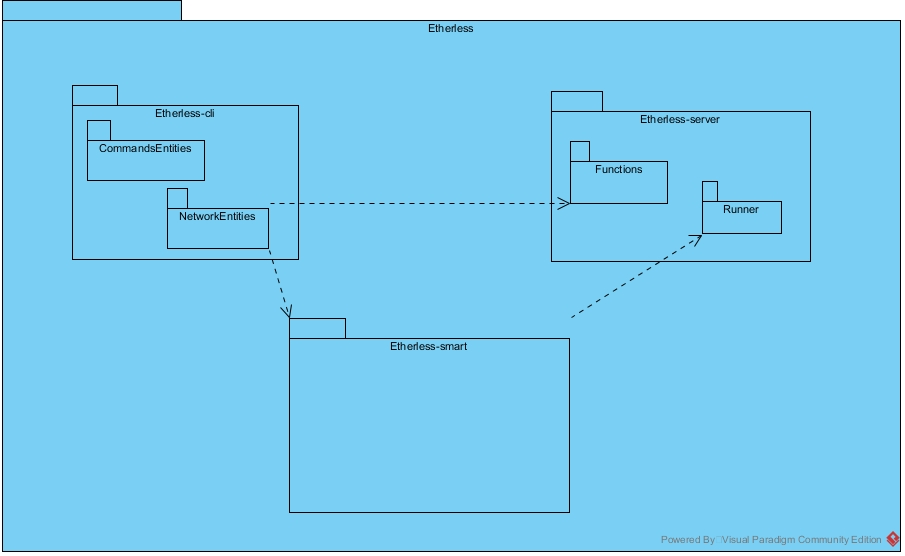
\includegraphics[width=\textwidth]{res/img/packageDiagram.jpg}
	\caption{Package diagram of Ethereum system}
\end{figure}
%In Typescript, the use of packages is not allowed, so the package diagram refers to project folders and its class dependencies.\\
%In the next section are explained all the possible communications between them.
\subsection{Communication}
The communication between these three components is key in understanding the dynamics of the software. We can identify three patterns that can be used based on what the neccesity is.
These three following sequence diagrams are informal and could not satisfy fully UML guidelines.
\subsubsection{Communication pattern 1}
Some functionalities that rely on this communication flow are: functions listing, get function details.
\begin{figure}[h]
	\centering
	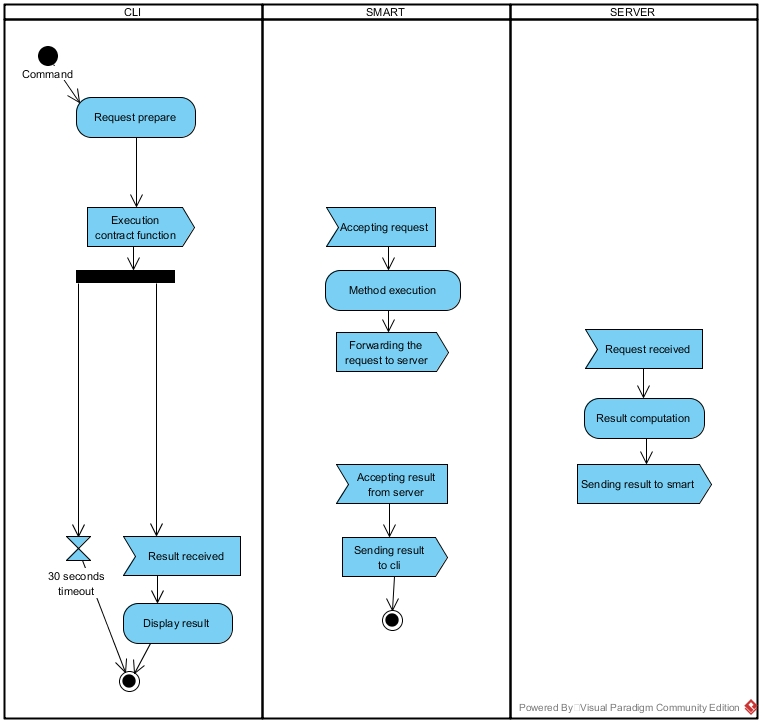
\includegraphics[width=0.8\textwidth]{res/img/pattern1.jpg}
	\caption{Communication pattern 1 overview}
\end{figure}
\noindent When a user launches a commands that requires the retrivial of information from the smart contract, a contract call is initiated. When the response is received, it gets displayed to the user through the command line window.\newline 

\subsubsection{Communication pattern 2}
In some cases the smart component will need to speak directly to the server component. Since smart contracts are unable to perform external calls, the only mean of communication is through Ethereum events. There is a part of etherless-server that is always listening for network events and, once captured, an adeguate response is computed and sent back to the contract (via contract call).\newline Since the communication between the smart and server components is asynchronous , events are used to get back to the cli components as final step.
\begin{figure}[!h]
	\centering
	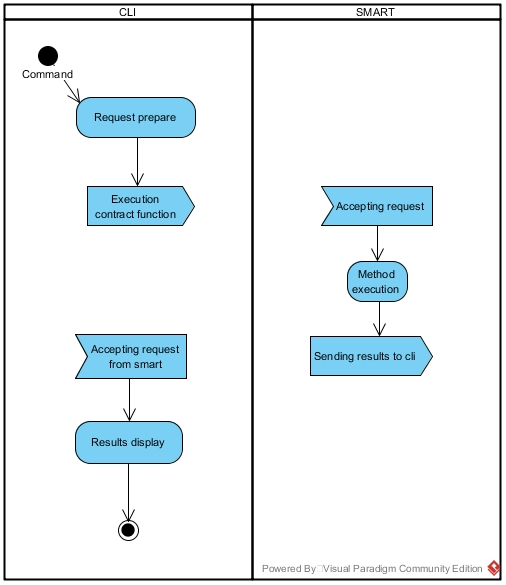
\includegraphics[width=0.8\textwidth]{res/img/pattern2.jpg}
	\caption{Communication pattern 2 overview}
\end{figure}
Some functionalities that rely on this communication flow are: function creation;
\subsubsection{Communication pattern 3}
There might be cases when a resource needs to be deployed to the server component and after getting a successful response, the contract can be updated.
\begin{figure}[!h]
	\centering
	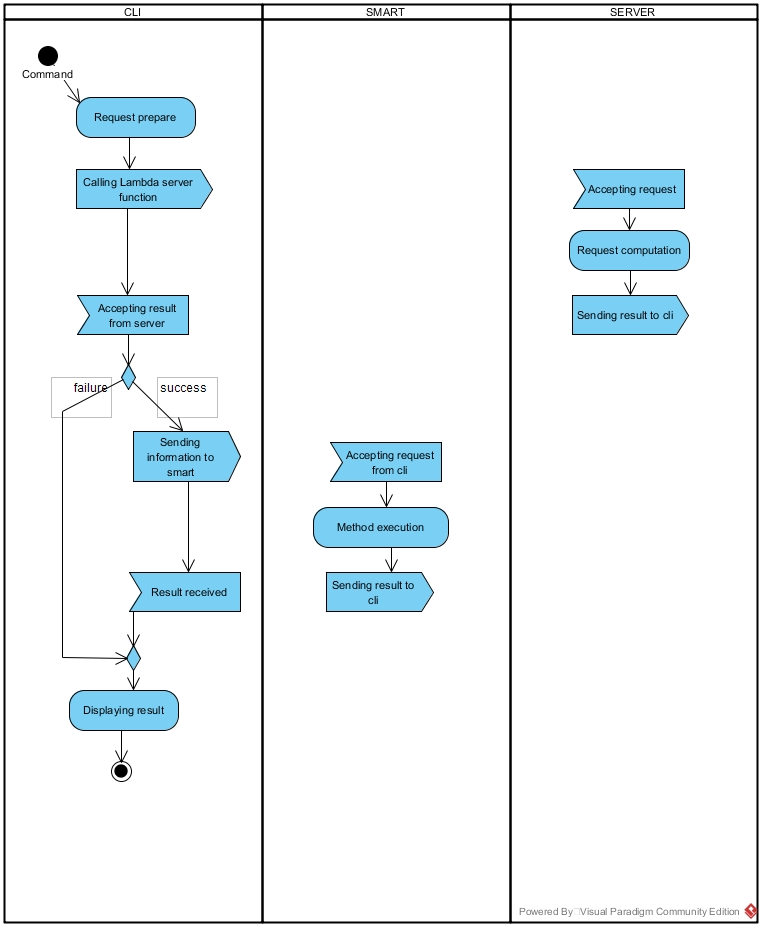
\includegraphics[width=0.8\textwidth]{res/img/pattern3.jpg}
	\caption{Communication pattern 3 overview}
\end{figure}
Some functionalities that rely on this communication flow are: function remote execution; 